\section{Results}
\paragraph{Accuracy on independently fitted bases.}
Table~\ref{tab:accuracy} compares policies selected on noisy validation; Figure~\ref{fig:accuracy_gain} shows gains relative to each base. Early-5 with base features raises CIFAR-100N accuracy from 70.12\% to 71.08\% on base seed 42 and from 69.23\% to 70.28\% on base seed 43. On CIFAR-10N Worse, it raises accuracy from 88.84\% to 90.16\%; uniform TTA obtains 89.29\%. All three Early-5 heads within each base have positive nominal paired gain intervals relative to that base (Appendix~\ref{app:intervals}). These repetitions distinguish a gain on two CIFAR-100N base initializations from three heads fitted to one base.
\begin{table}[t]
\centering\small
\caption{Test accuracy (\%). Parentheses in column headings identify base seeds. Mean $\pm$ sample standard deviation is over three head initializations on the same base; static scores have no head-seed variation. Each method selects its own view budget and temperature on noisy validation.}
\label{tab:accuracy}
\begin{tabular}{lccc}
\toprule
Method & C100 (42) & C100 (43) & C10 Worse (42) \\
\midrule
Base & 70.12 & 69.23 & 88.84 \\
Uniform TTA & 70.15 & 69.26 & 89.29 \\
MSP weighting & 70.15 & 69.26 & 89.27 \\
Gap weighting & 70.15 & 69.23 & 89.27 \\
Entropy weighting & 70.15 & 69.26 & 89.30 \\
Early-5, ResNet18 & 70.41 $\pm$ 0.12 & 69.32 $\pm$ 0.09 & 90.01 $\pm$ 0.17 \\
Static, base features & 70.35 $\pm$ 0.10 & 69.27 $\pm$ 0.01 & 89.19 $\pm$ 0.13 \\
History-50, base features & 70.46 $\pm$ 0.18 & 69.93 $\pm$ 0.09 & 89.01 $\pm$ 0.31 \\
Early-5, base features & 71.08 $\pm$ 0.24 & 70.28 $\pm$ 0.13 & 90.16 $\pm$ 0.02 \\
\bottomrule
\end{tabular}

\end{table}

\begin{figure}[t]
\centering
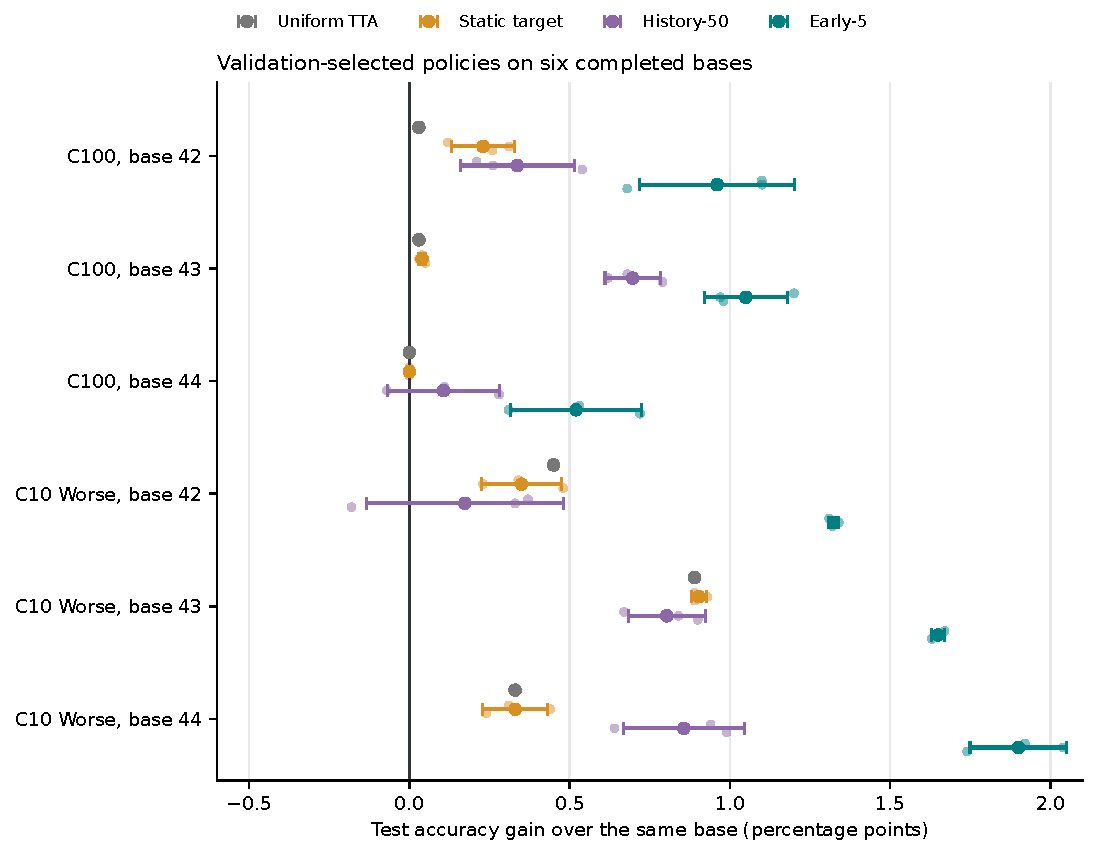
\includegraphics[width=\linewidth]{figures/accuracy_gain.pdf}
\caption{Accuracy gain over each corresponding base. Large dots and bars show the mean and sample standard deviation across three head seeds; small dots show individual heads. Bars do not estimate base-training uncertainty. Uniform TTA has no head. Each method selects its own view count and temperature on noisy validation.}
\label{fig:accuracy_gain}
\end{figure}

\paragraph{Target construction with matched heads.}
With base features, static-margin regression obtains 70.35\%, 69.27\%, and 89.19\% in the three runs, respectively. Early-5 obtains 71.08\%, 70.28\%, and 90.16\% with the same head architecture and policy-search procedure. The difference is therefore not explained solely by adding a trainable scalar head. It does not distinguish temporal information from the different augmentation and measurement conditions used to construct the targets. These are comparisons of the complete validation-selected policies; their selected temperatures and sometimes view budgets differ. The available paired intervals compare against base or same-view TTA, rather than directly against the static head, so we report the static contrast as a point-estimate comparison.

\paragraph{Early summaries and feature sources.}
The initial CIFAR-100N seed-42 window study is reported in Table~\ref{tab:windows} and Figure~\ref{fig:history_windows}. The first ten epochs give the highest observed test accuracy in that sweep, while the last five epochs and the full-history mean are weaker. This sweep is exploratory and does not select an optimal window using test accuracy. The primary Early-5 target also coincides with the cross-entropy warmup; later epochs use a different loss. Thus the window effect combines learning time and the loss schedule.

For Early-5, replacing ResNet18 features with selected-base features changes accuracy from 70.41\% to 71.08\% on CIFAR-100N seed 42, from 69.32\% to 70.28\% on seed 43, and from 90.01\% to 90.16\% on CIFAR-10N. Both encoders are fixed during head training, but their pretraining and task adaptation differ. This comparison supports using the selected base representation under this recipe; it does not isolate encoder architecture from adaptation.
\begin{table}[t]
\centering\small
\caption{Exploratory history-window study on CIFAR-100N, base seed 42. Accuracy is in percent; AUROC detects original-view base errors. Entries average three head seeds. All targets use scalar regression.}
\label{tab:windows}
\begin{tabular}{lrrrr}
\toprule
Target & R18 acc. & R18 AUROC & Base acc. & Base AUROC \\
\midrule
First 2 & 70.20 & 0.7391 & 70.88 & 0.8053 \\
First 5 & 70.41 & 0.7472 & 71.08 & 0.8307 \\
First 10 & 70.33 & 0.7414 & 71.25 & 0.8330 \\
First 20 & 70.26 & 0.7164 & 70.98 & 0.7920 \\
All 50 & 70.28 & 0.6599 & 70.46 & 0.7112 \\
Last 5 & 70.19 & 0.5641 & 70.23 & 0.5932 \\
Static checkpoint & 70.16 & 0.7021 & 70.35 & 0.8045 \\
\bottomrule
\end{tabular}

\end{table}

\begin{figure}[t]
\centering
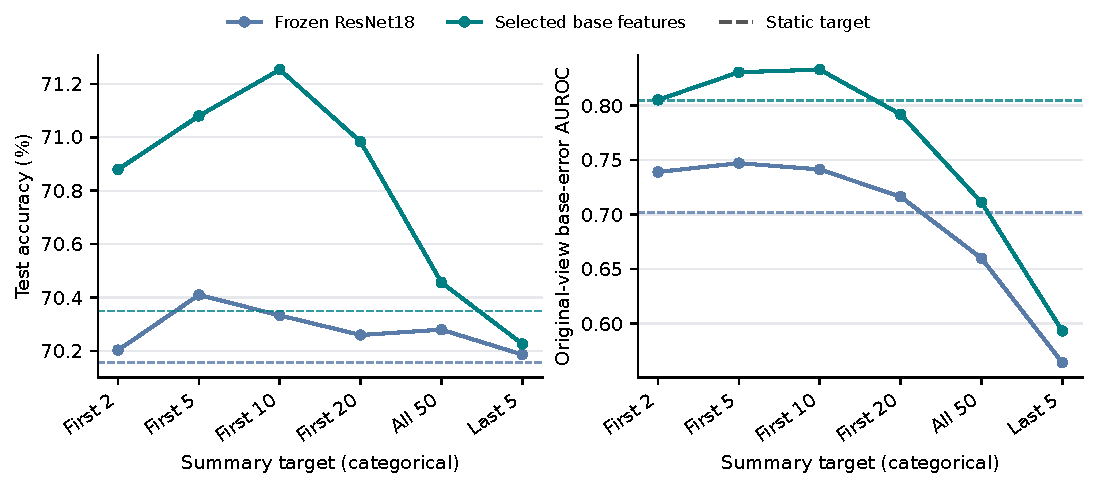
\includegraphics[width=\linewidth]{figures/history_windows.pdf}
\caption{Exploratory targets on CIFAR-100N, base seed 42. Points average three heads. Dashed lines show the static target for each feature source. Horizontal positions are categorical, not an epoch-time axis. Early-5 coincides with the cross-entropy warmup; the figure does not isolate learning time from the loss schedule or checkpoint timing.}
\label{fig:history_windows}
\end{figure}

\paragraph{Error ranking and calibration.}
Early-5 with base features increases error AUROC from MSP's 0.8124 to 0.8307 and from 0.8222 to 0.8326 for the two CIFAR-100N bases, and from 0.8764 to 0.9064 for CIFAR-10N. These are original-view error rankings, separate from the gains in aggregated prediction accuracy. On CIFAR-10N, mean ECE changes from 0.2847 to 0.2756 and NLL from 0.6203 to 0.5903. On CIFAR-100N, Early-5 worsens both ECE and NLL relative to each original-view base. Entropy weighting has better CIFAR-10N calibration than Early-5 despite lower accuracy. Full calibration results appear in Appendix~\ref{app:calibration}.

\paragraph{Ensembles and computational cost.}
A fixed original-view average of CIFAR-100N bases 42 and 43 reaches 73.01\%, exceeding either base with Early-5 weighting. Its nominal paired gain over base 42 is 2.89 points, with interval $[2.32,3.50]$. The comparison uses a different inference budget: the ensemble evaluates two bases once each, whereas the selected Early-5 policies evaluate one base on five views for CIFAR-100N and ten views for CIFAR-10N. There is therefore no demonstrated latency or forward-pass advantage over this two-base ensemble. Relative to uniform TTA at the same number of views, base-feature reuse avoids a second image encoder but adds PCA and the head.

Training cost includes the 50-epoch base run, trajectory recording, feature extraction, PCA, and head fitting. The experiments fit multiple controls and head seeds, so campaign wall time is not the cost of fitting a single deployment head. Storage for 45,000 float32 margins over 50 epochs alone is 9 MB in decimal units; cached features, weights, and predictions add further storage. The head contains $139{,}777+32C$ trainable parameters for $C$ classes. Hardware-matched end-to-end latency, memory, and training-overhead measurements are needed to quantify the deployment tradeoff.

